%% ============================================================
%%  HoneyIQ — Presentation Slides (Revised Edition, unified deck)
%%  Merges the original 14-frame deck with the extensions addendum
%%  into one coherent narrative. Compile: pdflatex slides
%%
%%  Figures expected in ../thesis-01/latex/figures/
%%  Copy or symlink that directory next to this file as figures/
%% ============================================================
\documentclass[aspectratio=169, 12pt]{beamer}

%% ── Theme ────────────────────────────────────────────────────
\usetheme{Madrid}
\usecolortheme{seahorse}
\setbeamertemplate{navigation symbols}{}
\setbeamertemplate{footline}[frame number]

%% ── Packages ─────────────────────────────────────────────────
\usepackage[utf8]{inputenc}
\usepackage[T1]{fontenc}
\usepackage{lmodern}
\usepackage{graphicx}
\graphicspath{{../thesis-01/latex/figures/}{figures/}}
\usepackage{booktabs}
\usepackage{multirow}
\usepackage{amsmath, amssymb}
\usepackage{xcolor}
\usepackage{tikz}
\usetikzlibrary{arrows.meta, positioning, shapes.geometric}

%% ── Colours ──────────────────────────────────────────────────
\definecolor{honeyblue}{RGB}{0,70,127}
\definecolor{honeyorange}{RGB}{220,100,30}
\definecolor{honeygrey}{RGB}{80,80,80}
\definecolor{alertred}{RGB}{180,30,30}
\definecolor{safegreen}{RGB}{30,130,80}

\setbeamercolor{title}{fg=white, bg=honeyblue}
\setbeamercolor{frametitle}{fg=white, bg=honeyblue}
\setbeamercolor{block title}{fg=white, bg=honeyblue}
\setbeamercolor{block title alerted}{fg=white, bg=alertred}
\setbeamercolor{block title example}{fg=white, bg=safegreen}

%% ── Metadata ─────────────────────────────────────────────────
\title[HoneyIQ]{%
  \textbf{HoneyIQ}\\
  \large Adaptive Honeypot Management\\
  Using a Stage-Escalation Decision Matrix}
\subtitle{MSc Dissertation Presentation --- Revised Edition:\\
  Traffic Realism, Escalation Tracking, and Auditable Dynamic Response}
\author{G.W.P.\ Chamikara \\ \small Student ID: 239149P}
\institute{%
  Department of Computer Science \& Engineering\\
  Faculty of Engineering}
\date{August 2026}

%% ============================================================
\begin{document}

%% ── Title ────────────────────────────────────────────────────
\begin{frame}
  \titlepage
\end{frame}

%% ── Outline ──────────────────────────────────────────────────
\begin{frame}{Overview}
  \tableofcontents
\end{frame}

%% ============================================================
\section{The Problem}

\begin{frame}{The World Has a Hacker Problem}
  \begin{columns}[T]
    \begin{column}{0.5\textwidth}
      \begin{alertblock}{Scale}
        \begin{itemize}
          \item Cybercrime cost \textbf{USD 8 trillion} in 2023
          \item Projected \textbf{USD 10.5 trillion/year} by 2025
          \item Nation-state groups, criminal syndicates, automated malware
        \end{itemize}
      \end{alertblock}
      \vspace{0.4cm}
      \begin{block}{Pattern}
        Hackers don't just \emph{attack} --- they \textbf{campaign}.\\
        They follow a structured playbook across days or weeks before causing damage.
      \end{block}
    \end{column}
    \begin{column}{0.45\textwidth}
      \begin{block}{Why current defences fall short}
        \begin{itemize}
          \item \textbf{Signature IDS}: blind to new techniques
          \item \textbf{Anomaly detectors}: too many false alarms
          \item \textbf{Static honeypot rules}: attacker learns to avoid triggers
        \end{itemize}
      \end{block}
    \end{column}
  \end{columns}
\end{frame}

%% ============================================================
\section{Background: Honeypots and the Kill Chain}

\begin{frame}{What is a Honeypot?}
  \begin{center}
    \Large\textbf{A decoy system --- designed to be attacked.}
  \end{center}
  \vspace{0.3cm}
  \begin{columns}[T]
    \begin{column}{0.48\textwidth}
      \begin{exampleblock}{Why honeypots work}
        \begin{itemize}
          \item Any interaction is \emph{inherently suspicious}\\
                (no legitimate user should be there)
          \item Zero risk to production assets
          \item Attacker reveals their tools and methods
        \end{itemize}
      \end{exampleblock}
    \end{column}
    \begin{column}{0.48\textwidth}
      \begin{alertblock}{The open question}
        \emph{How should the honeypot respond once an attacker is detected?}
        \begin{itemize}
          \item Stay quiet and watch? $\to$ miss escalation
          \item Block immediately? $\to$ lose intelligence
          \item Feed false data? $\to$ waste attacker resources
        \end{itemize}
      \end{alertblock}
    \end{column}
  \end{columns}
\end{frame}

\begin{frame}{Hackers Follow a Playbook: The Cyber Kill Chain}
  \begin{table}
    \centering
    \begin{tabular}{clp{5.5cm}}
      \toprule
      \textbf{Step} & \textbf{Phase} & \textbf{What the attacker does} \\
      \midrule
      1 & Reconnaissance       & Scans the network, finds targets \\
      2 & Weaponization        & Builds the attack tool \\
      3 & Delivery             & Sends the weapon (e.g.\ phishing) \\
      4 & Exploitation         & Breaks into a system \\
      5 & Installation         & Plants a back door \\
      6 & Command \& Control   & Phones home to their server \\
      7 & Actions on Objectives & Steals data, destroys files \\
      \bottomrule
    \end{tabular}
  \end{table}
  \vspace{0.3cm}
  \begin{center}
    \textcolor{honeyorange}{\textbf{Knowing which step the attacker is on tells you exactly how dangerous they are right now.}}
  \end{center}
\end{frame}

%% ============================================================
\section{HoneyIQ System Design}

\begin{frame}{HoneyIQ at a Glance}
  \begin{center}
    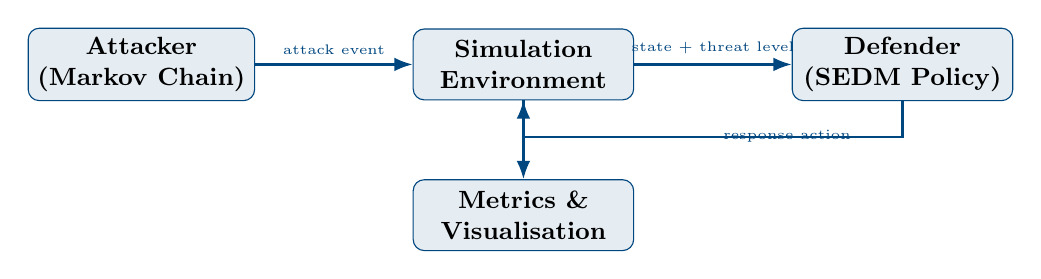
\begin{tikzpicture}[
        node distance=1.4cm,
        box/.style={rectangle, rounded corners, draw=honeyblue, fill=honeyblue!10,
                    minimum width=2.8cm, minimum height=0.9cm, align=center,
                    font=\small\bfseries},
        arrow/.style={-Latex, thick, color=honeyblue}
      ]
      \node[box] (atk)  {Attacker\\(Markov Chain)};
      \node[box, right=2.0cm of atk] (env)  {Simulation\\Environment};
      \node[box, right=2.0cm of env] (def)  {Defender\\(SEDM Policy)};
      \node[box, below=1.0cm of env] (met)  {Metrics \&\\Visualisation};

      \draw[arrow] (atk) -- node[above, font=\tiny] {attack event} (env);
      \draw[arrow] (env) -- node[above, font=\tiny] {state + threat level} (def);
      \draw[arrow] (def.south) -- ++(0,-0.45) -| node[right, font=\tiny, pos=0.25] {response action} (env.south);
      \draw[arrow] (env) -- (met);
    \end{tikzpicture}
  \end{center}
  \vspace{0.2cm}
  \begin{columns}[T]
    \begin{column}{0.48\textwidth}
      \begin{block}{Attacker module}
        Simulates 4 distinct hacker personalities using \textbf{probability chains}
        calibrated on real network data (UNSW-NB15).
      \end{block}
    \end{column}
    \begin{column}{0.48\textwidth}
      \begin{block}{Defender module}
        The \textbf{Stage-Escalation Decision Matrix (SEDM)} --- a transparent,
        printable lookup table that maps threat to response.
      \end{block}
    \end{column}
  \end{columns}
\end{frame}

\begin{frame}{Four Attacker Personalities}
  \begin{table}
    \centering
    \begin{tabular}{lp{3.5cm}p{5.0cm}}
      \toprule
      \textbf{Type} & \textbf{Behaviour} & \textbf{Why it matters for testing} \\
      \midrule
      Stealthy      & Slow, patient, avoids noise & Hardest to detect without false alarms \\
      Aggressive    & Fast, noisy, direct assault & Triggers many high-severity alerts \\
      Targeted      & Focused on one goal & Predictable path, but very dangerous \\
      Opportunistic & Scattered, tries everything & Represents typical automated attacks \\
      \bottomrule
    \end{tabular}
  \end{table}
  \vspace{0.2cm}
  \begin{center}
    \textcolor{honeygrey}{\small
    Each personality modifies the probability of moving between kill chain stages\\
    via \textbf{intent-specific transition matrices} --- producing qualitatively different attack campaigns.}
  \end{center}
\end{frame}

\begin{frame}{Session-Coherent Traffic Instead of Per-Step Noise}
  \begin{center}
    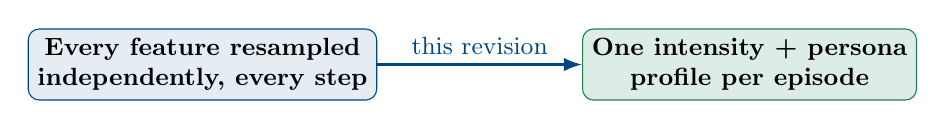
\begin{tikzpicture}[
        node distance=1.1cm,
        box/.style={rectangle, rounded corners, draw=honeyblue, fill=honeyblue!10,
                    minimum width=3.4cm, minimum height=0.9cm, align=center,
                    font=\small\bfseries},
      ]
      \node[box] (before) {Every feature resampled\\independently, every step};
      \node[box, right=2.6cm of before, fill=safegreen!15, draw=safegreen] (after)
        {One intensity + persona\\profile per episode};
      \draw[-Latex, thick, honeyblue] (before) -- node[above, font=\small] {this revision} (after);
    \end{tikzpicture}
  \end{center}
  \vspace{0.3cm}
  \begin{columns}[T]
    \begin{column}{0.48\textwidth}
      \begin{block}{Session intensity}
        $\iota \sim \text{Lognormal}(0, 0.35)$, applied to 8
        volume-shaped features (bytes, load, packet counts).
        TTL/window/duration untouched.
      \end{block}
    \end{column}
    \begin{column}{0.48\textwidth}
      \begin{block}{Three benign personas}
        \texttt{casual\_user} (70\%), \texttt{crawler} (20\%),
        \texttt{monitoring\_probe} (10\%) --- instead of one fixed
        ``NORMAL'' distribution.
      \end{block}
    \end{column}
  \end{columns}
  \vspace{0.2cm}
  \begin{center}
    \textcolor{honeygrey}{\small Classifier training data regenerated with fresh
    intensity/persona per sample --- retrained model: \textbf{99.4\% holdout accuracy}.}
  \end{center}
\end{frame}

\begin{frame}{Measuring Threat: The Composite Score}
  \begin{center}
    \Large $T = 0.45 \cdot \underbrace{S_{\text{type}}}_{\text{attack severity}}
            + 0.35 \cdot \underbrace{W_{\text{stage}}}_{\text{kill chain stage}}
            + 0.15 \cdot \underbrace{\rho}_{\text{escalation speed}}
            + 0.05 \cdot \underbrace{P_{\text{count}}}_{\text{attack volume}}$
  \end{center}
  \vspace{0.4cm}
  \begin{columns}[T]
    \begin{column}{0.48\textwidth}
      \begin{block}{Five threat bands}
        \begin{tabular}{ll}
          $T < 0.15$         & Benign \\
          $0.15 \le T < 0.35$ & Low \\
          $0.35 \le T < 0.55$ & Medium \\
          $0.55 \le T < 0.75$ & High \\
          $T \ge 0.75$        & Critical \\
        \end{tabular}
      \end{block}
    \end{column}
    \begin{column}{0.48\textwidth}
      \begin{exampleblock}{Why these weights?}
        \textbf{Attack severity} and \textbf{kill chain stage} carry the most information
        about real danger. Escalation rate adds forward-looking awareness.
        Volume prevents single-step detections from dominating.
      \end{exampleblock}
    \end{column}
  \end{columns}
\end{frame}

%% ============================================================
\section{The SEDM: A Transparent Decision Policy}

\begin{frame}{The Stage-Escalation Decision Matrix (SEDM)}
  \begin{center}
    \textbf{Two inputs $\Rightarrow$ one clear response. No black box.}
  \end{center}
  \vspace{0.2cm}
  \begin{table}
    \centering
    \small
    \begin{tabular}{lccc}
      \toprule
      \textbf{Kill Chain Stage} & \textbf{Low Risk} & \textbf{Medium Risk} & \textbf{High Risk} \\
      \midrule
      0 --- Reconnaissance  & ALLOW & LOG   & LOG   \\
      1 --- Weaponization   & LOG   & LOG   & TROLL \\
      2 --- Delivery        & LOG   & TROLL & TROLL \\
      3 --- Exploitation    & TROLL & BLOCK & BLOCK \\
      4 --- Installation    & BLOCK & BLOCK & ALERT \\
      5 --- Cmd \& Control  & BLOCK & ALERT & ALERT \\
      6 --- Objectives      & ALERT & ALERT & ALERT \\
      \bottomrule
    \end{tabular}
  \end{table}
  \vspace{0.2cm}
  \begin{columns}[T]
    \begin{column}{0.48\textwidth}
      \textbf{Override rules (checked in order):}\\
      \small
      R4: reputation $\ge 0.60 \to$ upgrade one level (\emph{new})\\
      R1: NORMAL traffic $\to$ always ALLOW\\
      R2: DoS or Worms $\to$ upgrade one level\\
      R3: high attack rate $\to$ upgrade one level
    \end{column}
    \begin{column}{0.48\textwidth}
      \begin{exampleblock}{Why this is powerful}
        Every single decision can be traced to a table cell.
        Security teams can read it, audit it, and change it
        \textbf{without any machine learning expertise.}
      \end{exampleblock}
    \end{column}
  \end{columns}
\end{frame}

\begin{frame}{What Each Response Means in Practice}
  \begin{table}
    \centering
    \begin{tabular}{clp{6.5cm}}
      \toprule
      \textbf{Response} & \textbf{Action} & \textbf{Plain English} \\
      \midrule
      ALLOW & Do nothing  & Normal traffic, no intervention \\
      LOG   & Record quietly & Something looks odd --- watch and note it \\
      TROLL & Feed false data & Keep the attacker busy with fake information to learn more \\
      BLOCK & Cut connection & Threat confirmed --- terminate immediately \\
      ALERT & Raise alarm   & Critical situation --- notify a human analyst now \\
      \bottomrule
    \end{tabular}
  \end{table}
  \vspace{0.3cm}
  \begin{center}
    \textcolor{honeygrey}{\small Responses escalate from \emph{observe} to \emph{engage} to \emph{contain} ---
    matching the attacker's own escalation through the kill chain.}
  \end{center}
\end{frame}

\begin{frame}{From a Hard Window to a Severity-Weighted EMA}
  \begin{columns}[T]
    \begin{column}{0.48\textwidth}
      \begin{block}{Before: sliding window}
        \[
          \rho_{\text{window}} = \frac{1}{|W|}\sum_{i \in W} \mathbb{1}[\text{attack}_i]
        \]
        \begin{itemize}
          \item Binary per step
          \item Hard cutoff at the window edge
          \item Recon probe = worm outbreak
        \end{itemize}
      \end{block}
    \end{column}
    \begin{column}{0.48\textwidth}
      \begin{exampleblock}{New: severity-weighted EMA}
        \[
          \rho^{(t)}_{\text{ema}} = \alpha\, s(\text{attack}_t) + (1-\alpha)\,\rho^{(t-1)}_{\text{ema}}
        \]
        \begin{itemize}
          \item Uses existing severity weights
          \item Smooth decay, no hard cutoff
          \item $\alpha = 0.15$
        \end{itemize}
      \end{exampleblock}
    \end{column}
  \end{columns}
  \vspace{0.3cm}
  \begin{alertblock}{Both signals always computed --- opt-in, not a replacement}
    \texttt{escalation\_mode="window"} stays the default everywhere.
    \texttt{RATE\_THRESHOLD} was calibrated against window semantics, so
    EMA mode needs its own validation pass before relying on R3's
    trigger behaviour. Measured: window R3 rate 44.7--90.0\% vs.\ EMA
    0.7--22.0\% across the four intents --- the two modes are not
    interchangeable without recalibration.
  \end{alertblock}
\end{frame}

\begin{frame}{Cross-Session Reputation: A New R4 Override}
  \begin{columns}[T]
    \begin{column}{0.52\textwidth}
      \begin{block}{The gap}
        Session state expires with its TTL (300s). A source IP that
        attacks, goes quiet, and comes back looks brand new.
      \end{block}
      \vspace{0.2cm}
      \begin{exampleblock}{ReputationTracker}
        Half-life-decayed offense score, per source IP, independent of
        individual sessions:
        \[
          \text{score}(t) = \text{score}(t_0)\cdot 0.5^{(t-t_0)/h}
        \]
        Default half-life: 6 hours.
      \end{exampleblock}
    \end{column}
    \begin{column}{0.44\textwidth}
      \begin{alertblock}{R4 --- checked before R1}
        Reputation $\geq 0.60 \Rightarrow$ upgrade one severity level,
        \textbf{even on a benign-looking event}.
      \end{alertblock}
      \vspace{0.2cm}
      \begin{center}
        \small\textcolor{honeygrey}{Fail2ban-style: once flagged,\\ stay flagged.\\[4pt]
        Measured: score crosses 0.60\\ at exactly the 4th offending\\
        visit (0.175/visit); R4 then\\ fires consistently on every\\
        subsequent benign-looking visit.}
      \end{center}
    \end{column}
  \end{columns}
\end{frame}

\begin{frame}{Bounded Threshold Adaptation --- Honestly Scoped}
  \begin{alertblock}{What we did \emph{not} build}
    \texttt{ESC\_LOW\_THRESHOLD} / \texttt{ESC\_HIGH\_THRESHOLD} adapt to
    \emph{nothing} --- they bucket a risk computed purely from a static
    Markov model. No live signal exists to tune them against, so we
    didn't pretend otherwise.
  \end{alertblock}
  \vspace{0.3cm}
  \begin{columns}[T]
    \begin{column}{0.48\textwidth}
      \begin{block}{What we did build}
        \texttt{AdaptiveThresholds}: a bounded deadband controller that
        nudges \texttt{RATE\_THRESHOLD} to keep R3's firing rate near a
        target --- an \textbf{alert-fatigue safety valve}, not a
        correctness fix.
      \end{block}
    \end{column}
    \begin{column}{0.48\textwidth}
      \begin{exampleblock}{Why the honesty matters}
        The only signal available is R3's \emph{own} trigger frequency
        --- not whether any trigger was right. There's no ground-truth
        feedback loop in this system. Framing this as ``learning
        correctness'' would be dishonest.
      \end{exampleblock}
    \end{column}
  \end{columns}
  \vspace{0.2cm}
  \begin{center}
    \textcolor{honeyblue}{\small Measured: the controller saturates to its
    bound under sustained high-rate traffic in both regimes tested; its
    effect is marginal under continuous attack (45.70\%$\to$44.40\%) but
    substantial under mixed traffic (7.60\%$\to$4.40\%).}
  \end{center}
\end{frame}

%% ============================================================
\section{Results}

\begin{frame}{Detection Performance: SEDM vs.\ Attacker Profiles}
  \begin{table}
    \centering
    \begin{tabular}{lcccc}
      \toprule
      \textbf{Attacker Profile} & \textbf{Detection Rate} & \textbf{False Alarms} & \textbf{Mean Reward} \\
      \midrule
      Stealthy      & \textbf{99.09\%} & 35.56\% & 1012 \\
      Aggressive    & \textbf{99.47\%} & 6.67\%  & 1091 \\
      Targeted      & \textbf{99.48\%} & 3.33\%  & 1127 \\
      Opportunistic & \textbf{99.41\%} & 15.00\% & 896  \\
      \midrule
      \textbf{Average} & \textbf{99.36\%} & \textbf{15.14\%} & \textbf{1031} \\
      \bottomrule
    \end{tabular}
  \end{table}
  \vspace{0.3cm}
  \begin{block}{Key insight}
    The SEDM was \textbf{never trained for any specific attacker type}.
    The same table, unchanged, achieves $>$99\% detection across all four
    profiles. \small (Original protocol: attack-only traffic, no benign
    steps --- see next slide for why that mattered.)
  \end{block}
\end{frame}

\begin{frame}{Why Almost No False Positives? Checking the Protocol}
  \begin{columns}[T]
    \begin{column}{0.48\textwidth}
      \begin{alertblock}{The gap in the original protocol}
        \texttt{benign\_ratio=0} in the primary evaluation: almost every
        step \emph{is} an attack, so there is almost nothing left for
        the classifier to misclassify \emph{as} an attack. A 0.00\% FPR
        under this protocol is a structural artefact, not evidence of a
        well-calibrated detector.
      \end{alertblock}
    \end{column}
    \begin{column}{0.48\textwidth}
      \begin{exampleblock}{What we changed}
        \begin{itemize}
          \item Re-ran the primary protocol with
                \textbf{\texttt{benign\_ratio=0.3}}, 50 episodes $\times$
                500 steps (up from 30$\times$200)
          \item Reported detection/FPR as \textbf{Wilson 95\% confidence
                intervals}, not bare point estimates
          \item Published raw attack/benign sample counts per intent
        \end{itemize}
      \end{exampleblock}
    \end{column}
  \end{columns}
  \vspace{0.4cm}
  \begin{block}{What we found}
    Original protocol: only 33--114 benign samples per intent --- a
    measured 0.00\% FPR whose 95\% CI upper bound reaches
    \textbf{10.4\%}. Revised protocol: 7{,}500+ benign samples per
    intent reveal a small, real, tightly-bounded FPR of
    \textbf{0.60--0.79\%} --- independently corroborated by Table 4.15's
    specificity figures (0.992--0.995). Detection rate is essentially
    unchanged (99.94--99.97\%).
  \end{block}
\end{frame}

\begin{frame}{SEDM vs.\ Deep Q-Network (AI Baseline)}
  \begin{columns}[T]
    \begin{column}{0.48\textwidth}
      \begin{block}{Deep Q-Network (DQN)}
        \begin{itemize}
          \item Neural network trained for 300 episodes
          \item $\approx$150,000 learning steps required
          \item Detection rate: $>$98.5\%
          \item \textcolor{alertred}{\textbf{Cannot explain decisions}}
          \item Specialises to training attacker only
        \end{itemize}
      \end{block}
    \end{column}
    \begin{column}{0.48\textwidth}
      \begin{exampleblock}{SEDM (This Work)}
        \begin{itemize}
          \item Lookup table, no training at all
          \item Ready to deploy instantly
          \item Detection rate: $>$99\%
          \item \textcolor{safegreen}{\textbf{Every decision is explainable}}
          \item Works across all four attacker profiles
        \end{itemize}
      \end{exampleblock}
    \end{column}
  \end{columns}
  \vspace{0.4cm}
  \begin{center}
    \large\textcolor{honeyblue}{\textbf{The SEDM matches AI performance --- with full human transparency.}}
  \end{center}
\end{frame}

\begin{frame}{Result Figures}
  \begin{columns}[T]
    \begin{column}{0.48\textwidth}
      \begin{center}
        
\includegraphics[width=\textwidth]{metric_comparison}\\
        \small Detection rate and false positive rate across all four profiles
      \end{center}
    \end{column}
    \begin{column}{0.48\textwidth}
      \begin{center}
        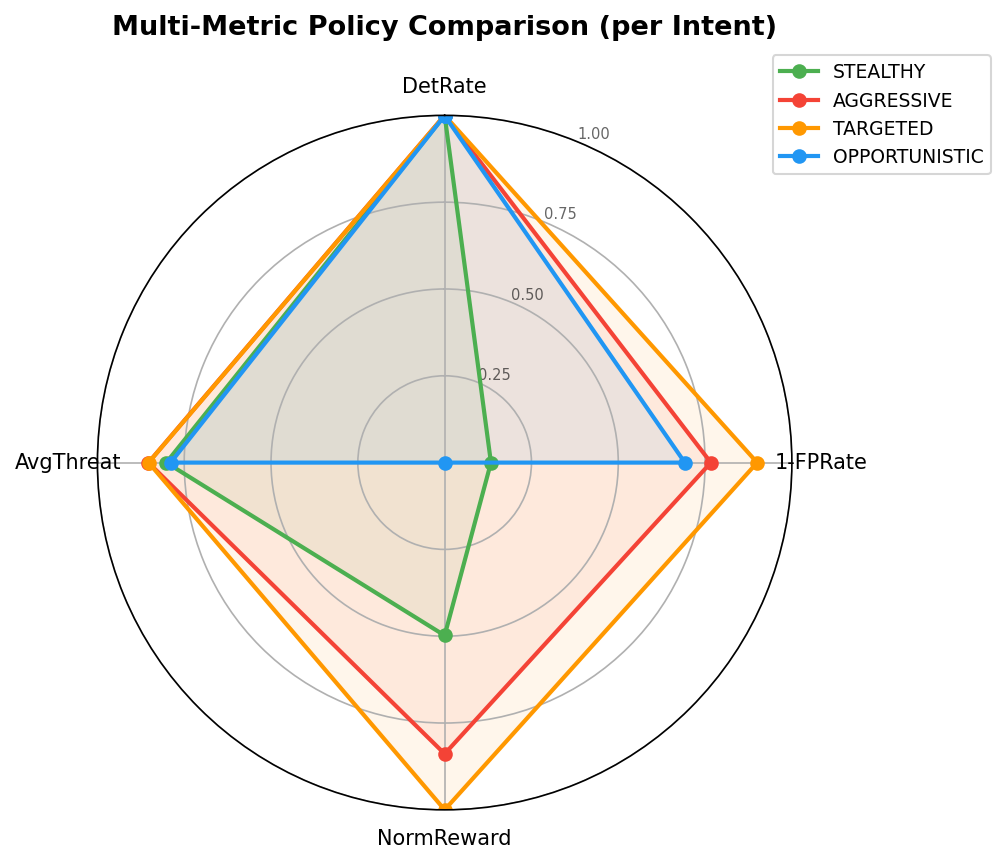
\includegraphics[width=\textwidth]{radar_comparison}\\
        \small Radar comparison: SEDM vs.\ DQN across metrics
      \end{center}
    \end{column}
  \end{columns}
\end{frame}

\begin{frame}{Why Does Stealthy Have More False Alarms?}
  \begin{columns}[T]
    \begin{column}{0.55\textwidth}
      \begin{itemize}
        \item Stealthy attackers spend more time at early kill chain stages (Reconnaissance, Analysis)
        \item Their traffic looks very similar to \emph{normal} traffic
        \item The SEDM correctly reacts to the elevated escalation risk --- but the ground truth says the step was borderline
        \item \textbf{This is a property of the scenario, not a flaw in the policy:} any system that is sensitive enough to catch stealthy attackers will produce more early-stage alarms
      \end{itemize}
    \end{column}
    \begin{column}{0.4\textwidth}
      \begin{alertblock}{Trade-off}
        \centering
        \vspace{0.2cm}
        High sensitivity\\
        $\updownarrow$\\
        More false alarms\\
        \vspace{0.2cm}
        \small This is fundamental to all intrusion detection --- HoneyIQ makes it \textbf{explicit and configurable}.
      \end{alertblock}
    \end{column}
  \end{columns}
\end{frame}

%% ============================================================
\section{Is a Learning-Based Approach More Practical?}

\begin{frame}{Revisiting DQN --- With Evidence We Already Have}
  \begin{columns}[T]
    \begin{column}{0.48\textwidth}
      \begin{alertblock}{What actually happened last time}
        \begin{itemize}
          \item Detection rate 87.6\% $\to$ 97.4\% in \emph{one episode}
          \item FPR pinned near \textbf{1.0} the whole time
          \item Learned ``almost never ALLOW,'' not real discrimination
          \item Trained on one intent only --- wouldn't generalise
        \end{itemize}
      \end{alertblock}
    \end{column}
    \begin{column}{0.48\textwidth}
      \begin{alertblock}{Why the eval harness makes this worse}
        Two independent, hard-to-catch label-alignment bugs inflated
        measured FPR by up to $10\times$ before being caught --- in code
        that only computed statistics \emph{after the fact}. A reward
        signal shapes learning on \emph{every step}.
      \end{alertblock}
    \end{column}
  \end{columns}
  \vspace{0.4cm}
  \begin{center}
    \large\textcolor{honeyblue}{\textbf{Conclusion: not practical right now.}
    The reputation override and the scoped threshold controller meet the
    same bar (Rudin, 2019) with none of the risk.}
  \end{center}
\end{frame}

\begin{frame}{If a Learning Component Is Ever Wanted}
  \begin{block}{Not a Q-network}
    A \textbf{small contextual bandit} choosing among 3--5 preset
    \texttt{RATE\_THRESHOLD} values --- nothing more ambitious than that.
  \end{block}
  \vspace{0.3cm}
  \begin{exampleblock}{The one prerequisite that doesn't exist yet}
    A reward needs a \textbf{trustworthy signal}: an analyst's own
    confirmed true/false-positive label on a logged decision. Decisions
    are already logged in full --- but nothing closes the loop from
    ``a human confirmed this was wrong'' back into a trainable signal.
  \end{exampleblock}
  \vspace{0.3cm}
  \begin{alertblock}{What we won't do}
    Manufacture a proxy signal (R1/R3 trigger rates) that \emph{looks}
    like learning without being grounded in ground truth --- that's the
    same trap the original DQN fell into.
  \end{alertblock}
\end{frame}

%% ============================================================
\section{Implications and Future Work}

\begin{frame}{Practical Takeaways for Security Teams}
  \begin{enumerate}
    \item \textbf{Start with an interpretable policy.}\\
          The SEDM is immediately deployable, auditable, and modifiable without data science expertise.

    \vspace{0.2cm}
    \item \textbf{Use the Kill Chain explicitly in your response logic.}\\
          The strong link between kill chain stage and correct response severity is a robust design principle.

    \vspace{0.2cm}
    \item \textbf{Add cross-session memory before adding intelligence.}\\
          A half-life-decayed reputation score closes a real gap (session TTL expiry) with a mechanism an analyst can hand-verify.

    \vspace{0.2cm}
    \item \textbf{Calibrate false alarm tolerance to your threat landscape.}\\
          Networks facing stealthy APTs need different thresholds than those facing automated scanners.

    \vspace{0.2cm}
    \item \textbf{Prefer a bounded controller to a learned one, until ground truth exists.}\\
          A deadband controller on trigger \emph{frequency} is honest about what it can and cannot fix; a DQN trained on the same absent ground truth would not be.
  \end{enumerate}
\end{frame}

\begin{frame}{Limitations and Future Work}
  \begin{columns}[T]
    \begin{column}{0.48\textwidth}
      \begin{alertblock}{Current limitations}
        \begin{itemize}
          \item Simulation only --- not tested on live networks
          \item Attacker does not adapt to defender responses
          \item Reputation constants ($h=6$h, threshold $=0.60$) are
                hand-chosen, not empirically validated
          \item R4-before-R1 trades a false-negative risk (missed
                genuine recovery) for a false-positive risk (stale
                flag) --- direction not yet validated against real
                attacker re-engagement data
          \item Adaptive threshold bound calibrated only for
                non-saturated traffic conditions
        \end{itemize}
      \end{alertblock}
    \end{column}
    \begin{column}{0.48\textwidth}
      \begin{exampleblock}{Natural next steps}
        \begin{itemize}
          \item Deploy against real honeypot logs
          \item Build an analyst-labelling pathway to enable a future,
                properly grounded learning component
          \item Model an attacker who reacts to the defender
          \item Extend to multi-node network topology
          \item Re-calibrate \texttt{RATE\_THRESHOLD} for EMA-mode
                escalation tracking
        \end{itemize}
      \end{exampleblock}
    \end{column}
  \end{columns}
\end{frame}

%% ============================================================
\section{Conclusion}

\begin{frame}{Six Extensions, All Additive}
  \begin{center}
    \small
    \begin{tabular}{p{4.2cm}p{5.4cm}p{2.4cm}}
      \toprule
      \textbf{Extension} & \textbf{Mechanism} & \textbf{Default} \\
      \midrule
      Session-coherent traffic & Per-episode intensity/persona & Always on \\
      Benign traffic diversity & Three weighted personas & Always on \\
      Randomised event payloads & Wordlist/jitter resolution & Always on \\
      Escalation tracking & Severity-weighted EMA & Opt-in \\
      Cross-session reputation & Half-life decay + R4 & Tracked; R4 opt-triggered \\
      Threshold adaptation & Bounded deadband controller & Opt-in \\
      \bottomrule
    \end{tabular}
  \end{center}
  \vspace{0.3cm}
  \begin{center}
    \textcolor{honeygrey}{\small Every new parameter defaults to the prior exact
    behaviour --- nothing breaks by standing still.}
  \end{center}
\end{frame}

\begin{frame}{Summary}
  \begin{block}{What was built}
    \textbf{HoneyIQ} --- a simulation framework with an intent-aware Markov attacker,
    an interpretable decision policy (SEDM), and --- in this revision ---
    session-coherent traffic, severity-weighted escalation tracking, and
    auditable dynamic response.
  \end{block}
  \vspace{0.3cm}
  \begin{columns}[T]
    \begin{column}{0.48\textwidth}
      \textbf{Core contributions:}
      \begin{enumerate}
        \item Coupled Markov attacker with 4 intent profiles
        \item Stage-Escalation Decision Matrix (SEDM), now with a
              cross-session reputation override (R4)
        \item Composite threat-level metric
        \item Session-coherent, persona-diverse synthetic traffic
      \end{enumerate}
    \end{column}
    \begin{column}{0.48\textwidth}
      \textbf{Key findings:}
      \begin{enumerate}
        \item $>$99\% detection --- no training required
        \item Transparent policy matches AI performance
        \item Structural cause of near-zero FPR identified and
              re-measured under mixed traffic with confidence intervals
        \item DQN re-examined and rejected on this project's own
              evidence, not assumption
      \end{enumerate}
    \end{column}
  \end{columns}
  \vspace{0.3cm}
  \begin{center}
    \large\textcolor{honeyblue}{\textbf{Effective. Explainable. Honestly evaluated.}}
  \end{center}
\end{frame}

\begin{frame}[plain]
  \begin{center}
    \vspace{1.5cm}
    {\Huge\textbf{Thank You}}\\[1cm]
    {\large HoneyIQ: Adaptive Honeypot Management\\
    Using a Stage-Escalation Decision Matrix\\
    \normalsize Revised Edition: Traffic Realism, Escalation Tracking,\\
    and Auditable Dynamic Response}\\[1cm]
    \begin{tabular}{rl}
      \textbf{Author:}     & G.W.P.\ Chamikara (239149P) \\
      \textbf{Supervisor:} & Dr.\ Thanuja Ambegoda \\
      \textbf{Degree:}     & MSc Data Science \& AI \\
      \textbf{Date:}       & August 2026 \\
    \end{tabular}\\[1cm]
    {\large\textit{Questions?}}
  \end{center}
\end{frame}

\end{document}
